\chapter{Shortest Path Problems}
\section{Introduction}
% Something about the importance of this problem family
\section{All pairs shortest path}
Here we see the power of exchanging the semiring for the first time. In this section we will use the tropical semiring $(\R \cup \{\infty\}, \min, +)$ and its induced matrix operations. But first we have to state the problem:
\begin{problem}[All pairs shortest path] 
    Given a directed weighted graph $G = (V, E)$ with $|V| = n$ and $|E| = m$ and its adjacency matrix $A$. Compute the length of the shortest path between every pair of nodes.
\end{problem}

\begin{lemma}
    Let $A \in \R^{n \times n}$ be an adjacency matrix. Then $(A^k)_{ij}$ holds the length of the shortest path with $k+1$ nodes between $v_i$ and $v_j$ for all $k \in \N$. 
\end{lemma}
\begin{proof}
    Let $D_k \in \R^{n \times n}$ ba a matrix such that $(D_k)_{ij}$ holds the length of the shortest path with $k+1$ nodes between $v_i$ and $v_j$. Thus we need to show that $A^k = D_k$ for all $k \in \N$ which we will do by induction. Namely, we need to show that (I) $D_0 = \imat_n$ and (II) $D_{k+1} = D_k \odot A$
    \begin{enumerate}
        \item[(I)] ...
        \item[(II)] ...
    \end{enumerate}
\end{proof}

\begin{lemma}
    Let $A \in \R^{n \times n}$ be an adjacency matrix of a directed weighted graph $G$. Then $G$ has no negative cycle $\Leftrightarrow$ 
    $$\sum_{k=0}^{n-1+q} A^k = \sum_{k=0}^{n-1} A^k \quad\forall q \in \N$$
\end{lemma}

\begin{corollary}
    A direct conclusion of the last lemma is that
    $$A^* = \sum_{k=0}^{\infty}A^k = \sum_{k=0}^{n-1}A^k$$
\end{corollary}

And $A^*$ solves our problem.

Our goal was more ambitious than just solving the problem. We wanted to state the solution in the language of Einsums. For that we need to go up one dimension. Let $R_{ijk} := A^{n-1}_{ij}$ be a tensor. Now we can rewrite $A^*$ as follows
$$A^*_{ij} = \sum_{k=0}^{n-1} A^k_{ij} = \sum_{k=1}^{n}A^{k-1}_{ij} = \sum_{k=1}^{n}R_{ijk}$$
This expression is allready in the necessary shape. The last step is to compute $R_{ijk}$. For that we need to define even more tensors: 
$$A^{(l)}_{ijk} := 
\begin{cases}
    A_{ij} & \textrm{if}\quad l \leq k\\
    \imat_{ij} & \textrm{else}   
\end{cases}
$$
As shown in Fig. \ref*{fig:shortest_path_tensor} we just need to multiply all matricies at each level together and than add the result up.

\begin{figure}[h]
    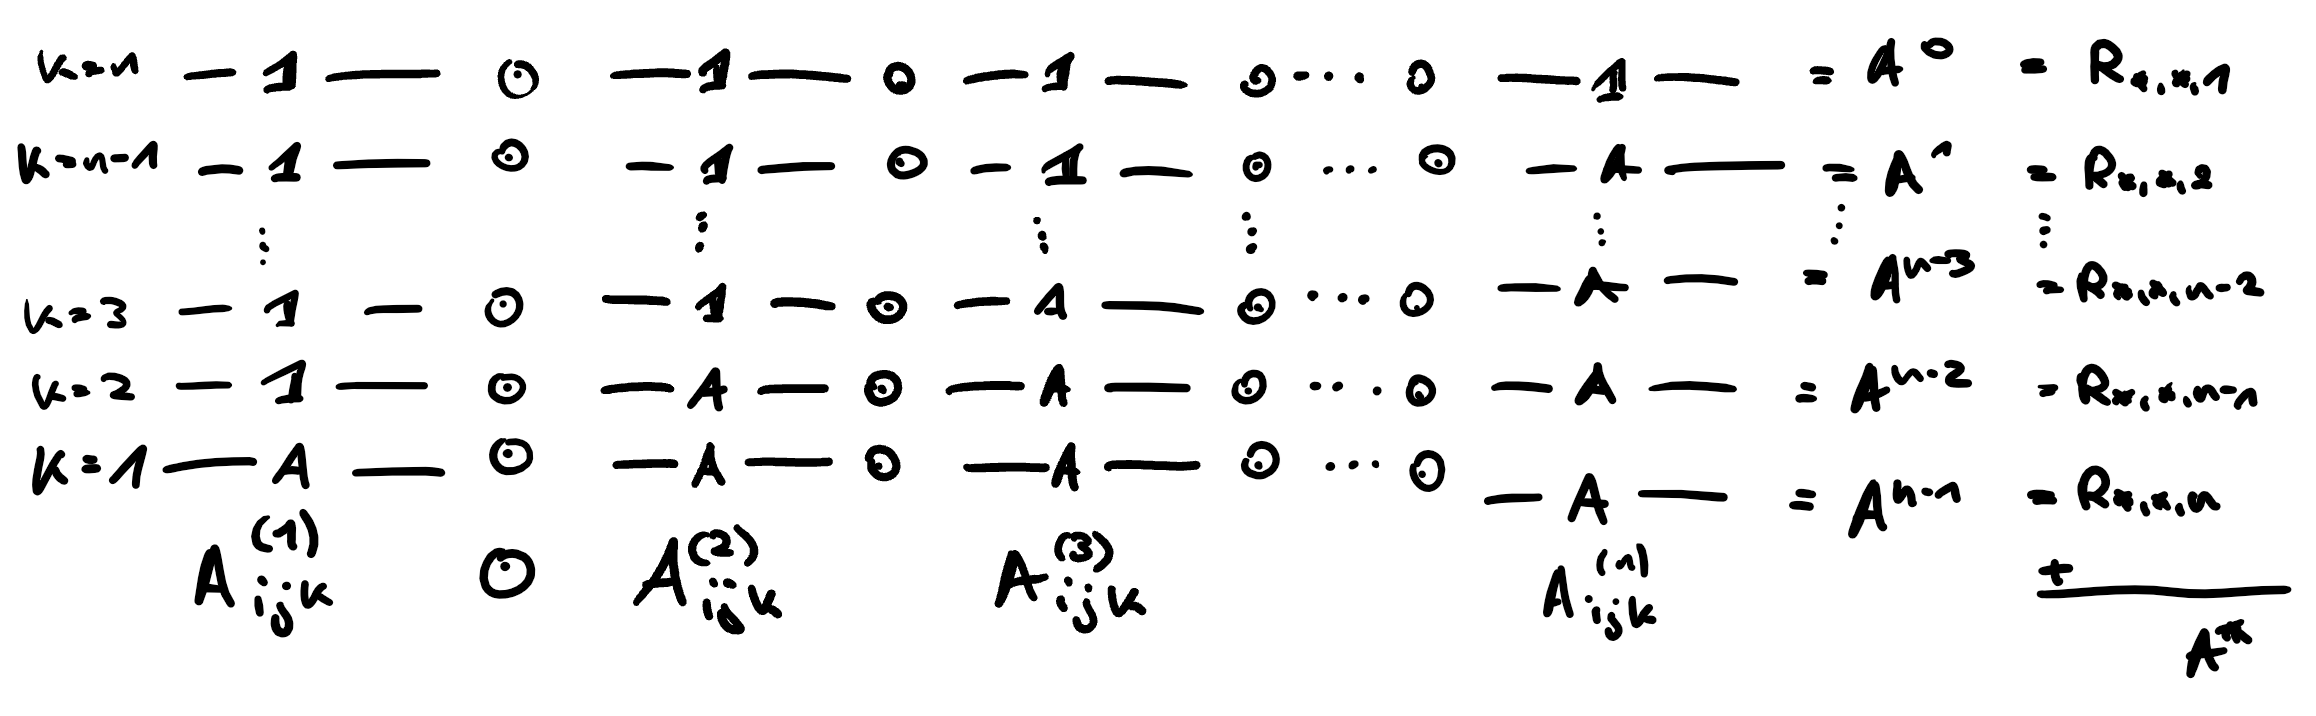
\includegraphics[width=\linewidth]{shortest_path_tensor.png}
    \caption{Visualized the shortest path tensors}
    \label{fig:shortest_path_tensor}
\end{figure}

The resulting expression comes out to be
$$A^*_{ij} = \sum_{k, t_1, \dots, t_{n-1} \in [n]} A^{(1)}_{it_1k}A^{(2)}_{t_1t_2k}A^{(3)}_{t_2t_3k}\dots A^{(n-1)}_{t_{n-2}t_{n-1}k}A^{(n)}_{t_{n-1}jk}$$
Which correspond to the Einsum string
$$it_1k, t_1t_2k, t_2t_3k, \cdots, t_{n-2}t_{n-1}k, t_{n-1}jk \to ij$$